
\documentclass[../thesis.tex]{subfiles}

\graphicspath{{./resources/} }
\begin{document}





\chapter{Evaluation}\label{chapter:eval}

\subfile{./05_evaluation/05_1_datasets.tex}

\section{Setup}
To evaluate the influence model created by the group sampling algorithm,
the accuracy of the trained model and its predictions of not yet seen configurations
need to be determined \cite{domingos2012few}.
The distance between the predicted values and the actual values
describes the accuracy of the model and can be used to compare different models on the
same dataset. For this, we need data, which was not used during the training of the model.
On our real-world examples, this can simply be done by randomly choosing samples from
all known configurations. In all tests in this chapter, we use a fixed test sample
size of 100 unless otherwise mentioned.
We repeat the test 20 times and work with the average measurement of those tests unless otherwise mentioned.

To evaluate models like the one created by our group sampling algorithm, several
well-known metrics exist. For simplicity, we use the MAPE metric to evaluate our model,
Although it might not be perfect, it is easy to understand for humans because it gives the models average
error as a percentage value.

\paragraph{Mean Absolute Percentage Error (MAPE)} describes the distance in per cent between
the actual value $A_{t}$ and the predicted value $P_{t}$ of all predictions n. MAPE
can't be used if the values contain zero, since it would result in a division by zero.

\begin{equation}
      MAPE = \frac{1}{n} \sum_{t=1}^{n}\left| \frac{A_t-P_t}{A_t} \right|
\end{equation}


% \paragraph{Mean Squared Error (MSE)} describes the average of the squared distance
% between the actual value $A_t$ and the predicted value $P_t$ for all predictions n.

% \begin{equation}
%       MSE = \frac{1}{n} \sum_{t=1}^{n}(A_t-P_t)^2
% \end{equation}


\subfile{05_evaluation/05_2_preliminary_tests.tex}
\subfile{05_evaluation/05_3_results.tex}



\section{Interpretation}\label{sec:evaluation:interpretation}


\subsection{Mitigation of constraints}
\paragraph{RQ1} How can we mitigate the effect of constraints on the configuration options for a group sampling approach?
\paragraph{}
In \autoref{sec:group_sampling:creation_of_groups} we described two methods to create groups of features to
implement a group sampling approach. We identified groups of mutually exclusive features as the major problem
in creating groups. The size of the smallest mutually exclusive group sets the maximum amount of groupings we
can create, without having potentially influential features in multiple groups.
Our solution is to weaken the constraint of having completely disjoint groups and allow mutually
exclusive features to be in multiple groups in one round of groupings.
While this allows us to create more groups, it limits our ability to make a statement about the influence of the feature.
In \autoref{sec:discussion:mutually_exclusive_group_size} we further discuss this solution and its influences.
In our approach, we need to specify the number of features a group has, which leads to unusable groups in our first approach.
Our tests show that more detailed knowledge about the feature model, especially mutually exclusive groups,
drastically improves the quality of the created groups.



\subsection{Effectiveness of group sampling}
\paragraph{RQ2} How effective is a group sampling algorithm compared to random sampling?
\paragraph{}
To answer this question, we compared the group sampling algorithm, and its method to create
a performance influence model, with a random sampling approach with linear regression.
In our real-world examples in \autoref{fig:evaluation:mape_real} we can see, that the group
sampling algorithm was mostly able to learn the influence of features. While the average
prediction accuracy was good, it lacks behind compared to a more straightforward approach with
random sampling and linear regression. Even though the group sampling algorithm seems to be
ahead of the random sampling approach on the JavaGC dataset, it was not able to make any meaningful
predictions about this dataset. The algorithm fails to identify any influential feature.
This is mainly because the JavaGC dataset only has feature interactions that influence the performance.
The group sampling algorithm, over multiple groupings, averages them down and
simply predicts the average of all seen measurements. On the other hand, the random sampling
algorithm with linear regression tries to fit the interactions once they appear in
a big enough sample size, which makes the model unusable.
In \autoref{sec:evaluation:interactions} we look at feature interactions in more detail.
In total, we can see that a group sampling approach to creating performance influence models
results in worse models than a more straightforward approach like distance-based sampling \cite{kaltenecker2019distance}
with linear regression. On our datasets with more features, the group sampling algorithm
performs even worse. 



\subsection{Scalability}\label{sec:evaluation:scalability}
\paragraph{RQ3} How scalable is group sampling?
\paragraph{}
We tested the scalability of group sampling using multiple synthetically created datasets.
In \autoref{fig:evaluation:mape_syn} we can see the results.
The group sampling algorithm struggles to create a meaningful model of the synthetic datasets.
Even though, in the synthetic datasets more independent variables are available to create groups.
The model does not improve with more samples, indicating an inability to learn more
information about the features from the samples provided.

\begin{figure}[h]
      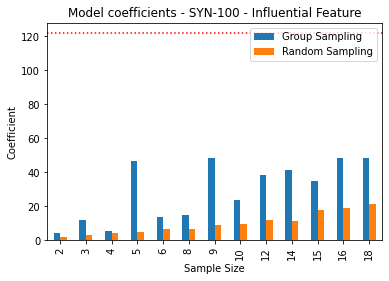
\includegraphics[width=0.5\textwidth]{graphs/syn-100-model-coefficient_sample_size.png}
      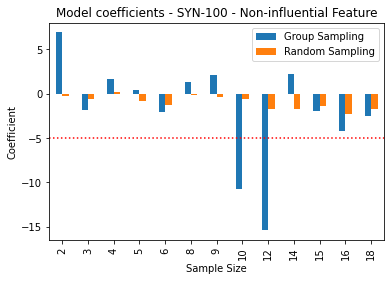
\includegraphics[width=0.5\textwidth]{graphs/syn-100-model-coefficient_sample_size_non_influential.png}
      \caption[Model coefficients - synthetic data with different sample sizes]{
            Resulting coefficients with different sample sizes.
      }\label{fig:evaluation:coefficients_influential}
\end{figure}

If we look at the coefficients calculated with the larger datasets, we can see why.
In \autoref{fig:evaluation:coefficients_influential} the coefficients for an influential and a non-influential feature
created by the group sampling algorithm
and by random sampling with linear regression are depicted. Since it is a synthetically generated
dataset we know the exact influence the feature should have. This influence is shown as the red dotted line.
The coefficients show us, that the group sampling algorithm was able to identify the influential feature in
the dataset with fewer samples even though it still wasn't able to estimate the influence correctly.
With the correct identification of the influential feature, the model should be more accurate. 
Nevertheless, the group sampling algorithm is not able to correctly identify the influence of non-influential features.
In the graph for the non-influential feature, we can see that it has a lot of variances when determining the influence of a non-influential feature.
With a high average error among non-influential features, the group sampling algorithm produces
worse predictions the more non-influential features are in the dataset. 
We further discuss the problem of inaccurate estimates on non-influential features in\autoref{sec:discussion:estimate}.



\subsection{Group sampling with interactions}\label{sec:evaluation:interactions}
\paragraph{RQ4} Can group sampling be used to effectively identify feature interactions and include them in the resulting model?
\paragraph{}

In order to answer if group sampling can identify feature interactions and include them in the model, 
we tested our approach described in \autoref{sec:group_sampling:interactions} on synthetically generated data.
As with RQ3 the model's prediction accuracy did not follow an obvious trend and did not perform very well.
In \autoref{fig:evaluation:interactions} we can see how the group sampling algorithm performed with the inclusion
of feature interactions as described in \autoref{sec:group_sampling:interactions}. 
The initial gain in accuracy in respect to the sample size is caused by the group sampling algorithm identifying 
the influential feature in the dataset and only a few interactions appearing of which, most likely, none are influential.
To explain the degrading performance with increasing sample size, it is, again, worth looking at the learned coefficients.
\autoref{fig:evaluation:interactions_coefficients} shows the coefficients of the models trained with the highest sample count. 

\begin{figure}[!h]
      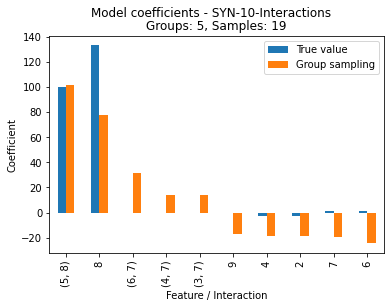
\includegraphics[width=0.5\textwidth]{graphs/syn-10-int-coef.png}
      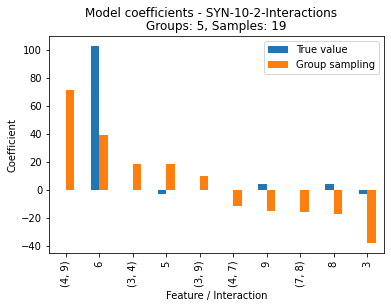
\includegraphics[width=0.5\textwidth]{graphs/syn-10-2-int-coef.png}
      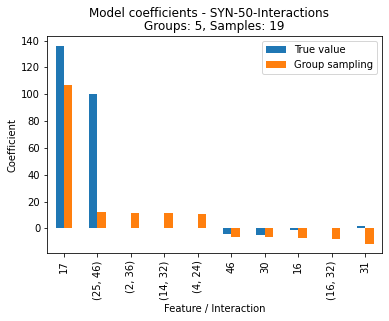
\includegraphics[width=0.5\textwidth]{graphs/syn-50-int-coef.png}
      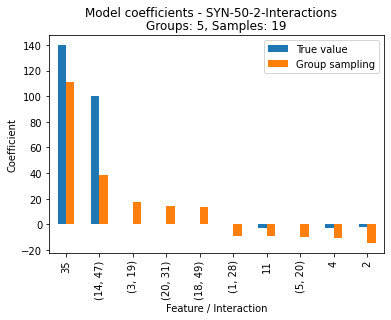
\includegraphics[width=0.5\textwidth]{graphs/syn-50-2-int-coef.png}
      \caption[Model coefficients - interactions on synthetic data]{
            Feature and interaction coefficients - Top 5 positively influential and top 5 negatively influential
      }\label{fig:evaluation:interactions_coefficients}
\end{figure}


While the group sampling algorithm was able to identify the influential feature in all datasets, it only
successfully identified the interaction in two out of four cases. A plausible explanation for this is that
the number of groupings is not enough for an influential interaction to appear in the samples to train the model.
We can also see a larger estimated influence in non-influential features and interactions. 
Since we treat interactions the same way as features, the average error on non-influential features and 
interactions make the model unreliable. We discuss a possible cause of the unreliable estimates on
non-influential features in \autoref{sec:discussion:estimate}.  



\end{document}


